\documentclass{article}
\usepackage[margin=1in]{geometry}
\usepackage{../common}
\usepackage{../pagesetup}
% **** IF YOU WANT TO DEFINE ADDITIONAL MACROS FOR YOURSELF, PUT THEM HERE:

\begin{document}

\lecture{3}{September 11}{Sasha Rush}{Christopher Mosch, Lindsey Brown, Ryan Lapcevic}{Multivariate Normal Distributions}

\subsection{Examples}
Multivariate gaussians are used for modeling in various applications, where knowing mean and variance is useful:
\begin{itemize}
\item{radar: mean and variance of approaching objects (like invading aliens)}
\item{weather forecasting: predicting the position of a hurricane, where the uncertainty in the storm's position increases for timepoints farther away}
\item{tracking the likely outcome of a sports game: last year's superbowl is an example of a failure of modeling with multivariate gaussians as the Patriots still won after a large Falcons' lead}
\end{itemize}

\subsection{Review: Eigendecomposition} 

Let $\v \Sigma$ be a square, symmetric matrix. Then its eigendecomposition is given by $\v\Sigma = \v U^T \v\Lambda \v U$, where $\v U$ is an orthogonal matrix and $\v\Lambda$ is a diagonal matrix. In the special case that $\v\Sigma$ is positive semidefinite (as is the case for covariance matrices), denoted $\v\Sigma \succeq 0$, all its eigenvalues are nonnegative, $\Lambda_{ii} \geq 0$, and we can decompose its inverse as $\v\Sigma^{-1} = \v U^T \v\Lambda^{-1}\v U$, where $\Lambda_{ii}^{-1} = 1/\Lambda_{ii}$.

\subsection{Multivariate Normal Distributions (MVNs)}
Let $X$ be a D-dimensional MVN random vector with mean $\v\mu$ and covariance matrix $\v\Sigma$, denoted $X \sim \mathcal{N}\left(\v\mu,\v\Sigma\right)$. Then the pdf of $X$ is
$$ p(x) = \left(2\pi\right)^{-D/2} |\v\Sigma|^{-1/2} \exp{[-\frac{1}{2}(x-\v\mu)^T\v\Sigma^{-1}(x-\v\mu)]}, $$
where for many problems we focus on the quadratic form $(x-\v\mu)^T\v\Sigma^{-1}(x-\v\mu)$ (which geometrically can be thought of as distance) and ignore the normalization factor $\left(2\pi\right)^{-D/2} |\v\Sigma|^{-1/2}$. The figure below plots the contours of a bivariate Normal for various $\v\mu$ and $\v\Sigma$ (in the figure, $\rho$ denotes the off-diagonal elements of $\v\Sigma$, given by the covariance of $x_1$ and $x_2$).

\begin{center}
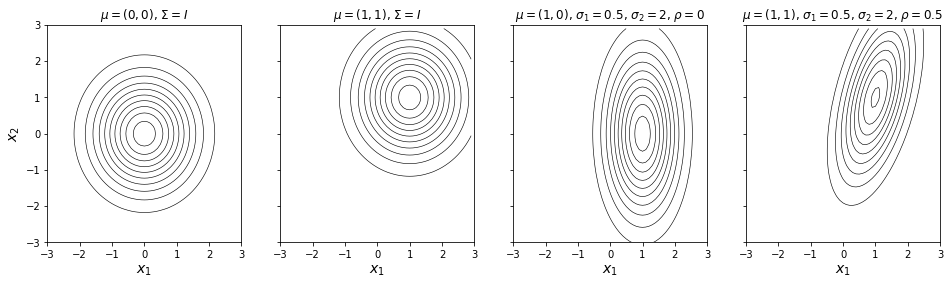
\includegraphics[width=\textwidth]{MVN_contour.png}
\end{center}

Note that we can decompose $\v\Sigma$ as
\begin{align*}
\v\Sigma &= (x-\v\mu)^T\v\Sigma^{-1}(x-\v\mu) \\
&= (x-\v\mu)^T\left(\v U^T \v\Lambda^{-1}\v U\right)(x-\v\mu) \\
&= (x-\v\mu)^T\left(\sum_d{\frac{1}{\lambda_d} U_d U^T}\right)(x-\v\mu) \\
&= \sum_d{\frac{1}{\lambda_d}(x-\v\mu)^T U_d U_d^T (x-\v\mu)},
\end{align*}
where $(x-\v\mu)^T U_d$ can be interpreted as the projection of $(x-\v\mu)$ onto $U_d$ (which can each be thought of as univariate gaussians), the eigenvector corresponding to the eigenvalue $\lambda_d$. Since $\v\Sigma$ is the weighted sum of the dot product of such projections (with weights being given by $1/\lambda_d$, which can be thought of as the scale $1/\sigma^2$), we can describe the MVN as tiling of univariates.

\subsubsection{Manipulating MVNs: Stretches, Rotations, and Shifts}
Let $x\sim\mathcal{N}(0,\v I)$ and $y = \v A x + \v b$. We want to consider two ways of obtaining the complete distribution of $y$.

\begin{itemize}
\item 'Overkill': We can perform a change of variables\footnote{A change of variables can be done in the following way: Let $y=f(x)$ and assume $f$ is invertible so that $x=f^{-1}(y)$. Then $p(y) = p(x)|dx/dy|$.  This is a technique which will be used often in this course}. Here, we have $x = \v A^{-1}$ and $|dx/dy| = \v |A^{-1}|$, leading to
\begin{align*}
p(y) &= \mathcal{N}\left(\v A^{-1}(y-\v b)|0,\v I\right)|\v A^{-1}| \\
&= \frac{1}{z}\exp{[(\v A^{-1}(y-\v b))^T(\v A^{-1}(y-\v b))]} \\
&= \frac{1}{z}\exp{[(y-\v b)^T(\v A^{-1})^T(\v A^{-1})(y-\v b)]} \\
&= \mathcal{N}(y|\v b,\v A\v A^T),
\end{align*}
where $z$ is the normalizing constant.
\item Using the properties of MVN, we know that $y$ is also MVN, so is completely specified by its mean and covariance matrix which can easily be derived,
$$ \E(y) = \E(\v A x + \v b) = \v A \E(x) + \v b \quad\quad \cov(y) = \v A \v A^T. $$
\end{itemize}

Thus, we can generate MVN from $\mathcal{N}(0,\v I)$ via the transformation $y = \v A x + \v b$, where we set $\v A = \v U \v \Lambda^{1/2}$, leading to $\v\Sigma_Y = \v U^T \v\Lambda \v U$. Then shifts are represented by $\v b$, stretches by $\v \Lambda$, and rotations by $\v U$.

\subsubsection{Detour: MVN in High-Dimensions ($D\gg 0$)}
Let $x$ be a D-dimensional random vector, distributed as $\mathcal{N}(0,I/D)$, where $I$ is the identity. The expected length of $x$ is given by
$$ \E\left(\lVert x \rVert^2\right) = \E\left(\sum_d{x_d^2}\right) = D\sigma_d^2 = 1, $$
which means that $x$ is expected to be on the boundary of a unit sphere centered at the origin. Moreover, the variance of the length is
$$ \text{var}\left({\lVert x \rVert}^2 \right) = D\cdot\left(\E(x^4) - \E\left(x^2\right)^2\right) = D\cdot(3\sigma^4-\sigma^4) = 2D/D^2 = 2/D$$
Thus, it is not only expected that $x$ lies on the boundary but as $D$ increases most of its realizations will in fact fall on the boundary\footnote{It is left as an exercise to show that this formula holds.  Hint: Use the fact that we assumed no covariance.}.

\subsubsection{Key Formulas for MVN: Marginalization and Conditioning}
Let $X \sim \mathcal{N}\left(\v\mu,\v\Sigma\right)$ with
$$ X = \begin{pmatrix}X_1\\X_2\end{pmatrix}, \quad 
\v{\mu} = \begin{pmatrix}\v{\mu}_1\\ \v{\mu}_2\end{pmatrix}, \quad
\v\Sigma = \begin{pmatrix}
\v\Sigma_{11} & \v\Sigma_{12} \\
\v\Sigma_{21} & \v\Sigma_{22}
\end{pmatrix}.
$$
Note that $\Sigma$ is written in block matrix form, rather than scalar entries.  It turns out that the marginals, $X_1$ and $X_2$, are also MVN, and their mean and covariance matrice are given by $\v\mu_1$ and $\v\Sigma_{11}$ and $\v\mu_2$ and $\v\Sigma_{22}$ respectively. A sketch of the proof is provided below.
$$ p(x_1) = \int_{x_2}{N(x|\v\mu,\v\Sigma)dx_2}, $$
which can be written as
$$ 0.5\int_{x_2}{\exp{\left[(x_1-\v\mu_1)^T\v\Sigma_{11}^{-1}(x_1-\mu_1) 
+ 2(x_1-\v\mu_1)^T\v\Sigma_{12}^{-1}(x_2-\mu_2) + 
(x_2-\v\mu_2)^T\v\Sigma_{22}^{-1}(x_2-\mu_2)\right]}dx_2}. $$
Note that this equals
$$ p(x_1)\int_{x_2}{p(x_2|x_1)dx_2}, $$
implying that $X_1\sim\mathcal{N}(\v\mu_1,\v\Sigma_{11})$. 

While the marginals have a simple form, the conditionals are more complicated.  (For a complete derivation, which requires matrix inversion lemmas, refer to Murphy.) It can be shown that $ X_1|X_2 \sim \mathcal{\v\mu_{1|2},\v\Sigma_{1|2}}$ with
$$ \v\mu_{1|2} = \v\mu_1+\v\Sigma_{12}\v\Sigma_{22}^{-1}(x_2-\v\mu_2), \quad
\v\Sigma_{1|2} = \v\Sigma_{11}-\v\Sigma_{12}\v\Sigma_{22}^{-1}\v\Sigma_{21}.$$
\subsubsection{Information Form}
An alternative formulation, called information form, uses the precision matrix (inverse variance) $\Lambda = \Sigma^{-1}$. Partitioning $\Lambda$ as
$$ \v\Lambda = \begin{pmatrix}
\v\Lambda_{11} & \v\Lambda_{12} \\
\v\Lambda_{21} & \v\Lambda_{22}
\end{pmatrix}, $$
the covariance matrices of the conditional distributions have a simple form. For example, the covariance matrix of $X_1$ given $X_2$ is $\Lambda_{1|2}=\Lambda_{11}$. However, the simplicity of the conditional precision comes at the cost of marginalization (which was simple when using $\Sigma$) becoming a more complicated expression (see Murphy subsection 4.3 for more details).

\end{document}



